% ! TeX program = pdflatex

% PACKAGES
\documentclass[12pt,oneside, a4paper]{book}
\usepackage[utf8]{inputenc}
\usepackage{commath, amsmath,amssymb,amsthm,mathtools,mathrsfs}
\usepackage[spanish]{babel}
\usepackage{setspace}
\usepackage{footnote}
\usepackage{minipage-marginpar}
\usepackage{dashbox}
\usepackage{dsfont}
\usepackage{hyperref}
\usepackage{bm}
\usepackage{indentfirst}
\usepackage{titlesec}
\usepackage{biblatex}
\addbibresource{bibliography.bib}




% COMMANDS
\newcommand{\HRule}{\rule{\linewidth}{0.5mm}}


\begin{document}
    


\begin{titlepage}
    \begin{center}
    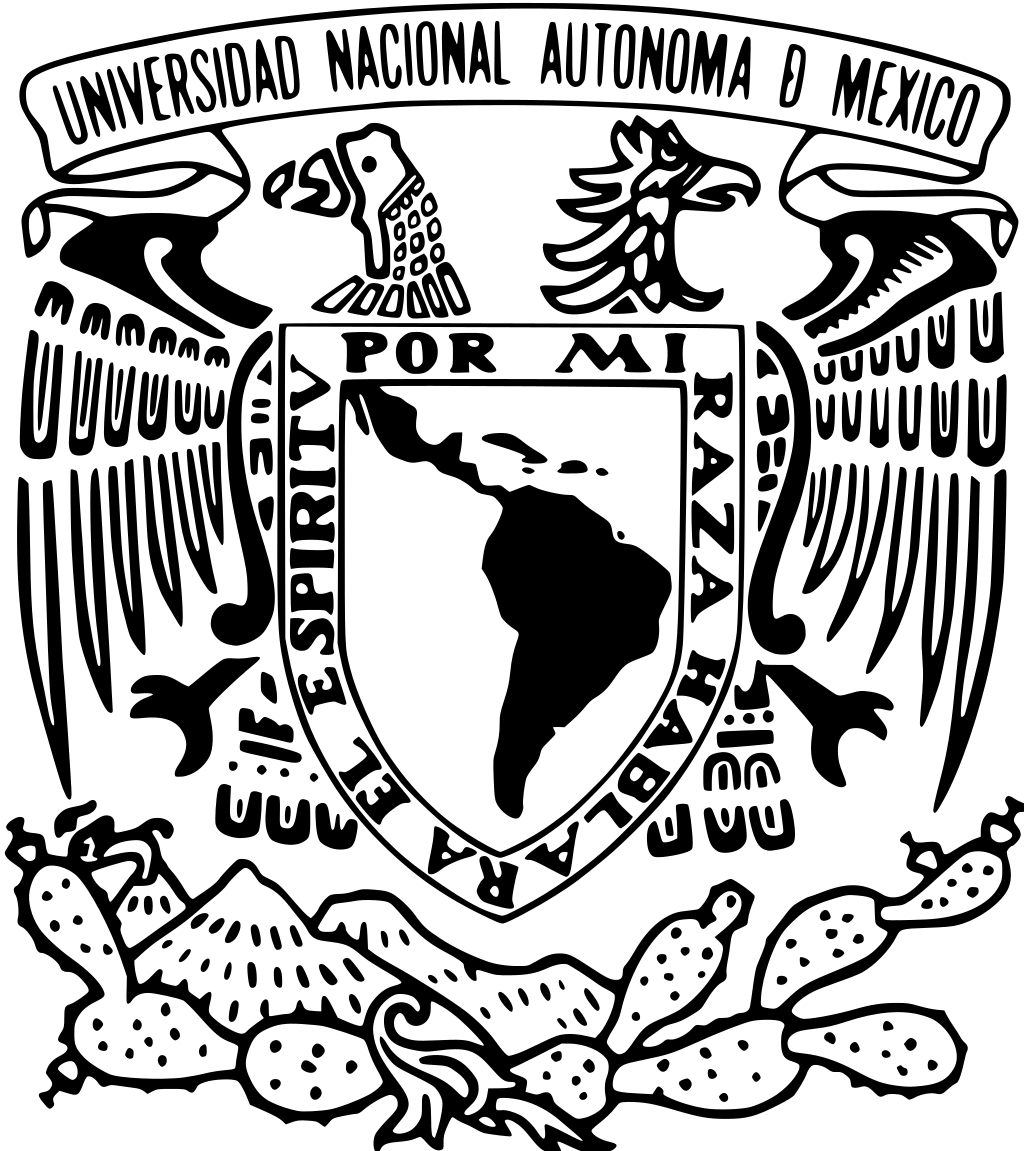
\includegraphics[width=0.25\textwidth]{resources/unam_escudo.png}~\\[2cm]
    \textsc{\huge Universidad Nacional Autónoma de México}\\[0.5cm]  
    \textsc{\LARGE Instituto de Matemáticas}\\[2cm]
    
    \HRule \\[0.5cm] 
    {\Huge \bfseries Interpretabilidad de los \\[1cm] Ataques Adversarios} \\[0.3cm] 
    \HRule \\[0.5cm]
    
    \textsc{\LARGE Reporte del Proyecto Final}\\[0.4cm]
    \textsc{\LARGE - Redes Neuronales - }\\[3cm]
    
    % Authors 

    {\Large
    \begin{tabular}{ccc}
        Aaron Kelley & \hspace{1.5in} & Rodrigo Fritz
    \end{tabular}
    }
    % {\Large \hspace{0.5in} \& Aaron Kelley\hspace{1.5in} }
    \vfill

    % Bottom of the page  
    {\Large 18 de junio, 2021}
    
    \end{center} 
\end{titlepage}

\section*{Abstract}
Abstract Goes here \\[1cm]

\noindent\textbf{Keywords}:  

\tableofcontents





\section{Introducción}
\cite{einstein}




\printbibliography





\end{document}


